\section{Results and Tests}

The testing of the energy consumption was done by measurement in the eAProfiler software.
While the program was running on the Development Board, input was provided, results measured and discussed.

Power consumption is minimal when the system idles, with the system in Deep Sleep mode (EM2) averaging $ 1.8 \mu Ah $. Power consumption during playback was at a continuous $ 2.0 mAh $.

\subsection{Startup}

When the program boots, a sound is played. The spike in power consumption \ref{fig:startuppower} is therefore expected, and the system quickly returns to idle consumption levels after the sound sample has finished playing.

\begin{figure}[H]
\centering
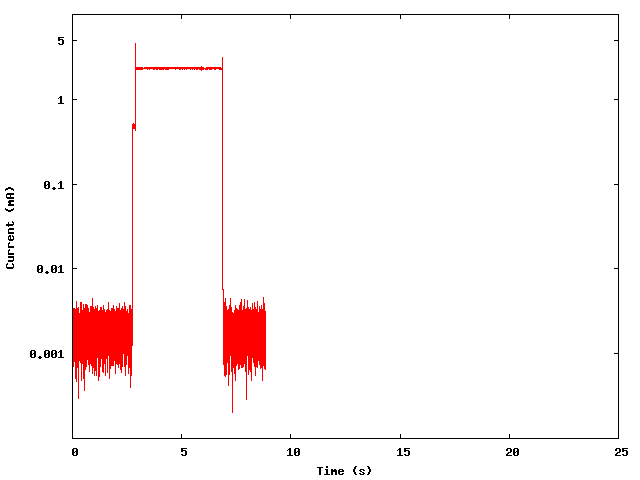
\includegraphics[width=0.75\textwidth]{data/startup.png}
\caption{Startup power consumption}
\label{fig:startuppower}
\end{figure}

\subsection{Playing music}

Figure \ref{fig:playpower} shows the power consumption of switching between different songs, and then playing that song.
It can be seen how the micro controller goes to sleep right after receiving the button interrupt, and after the song finishes playing.
Had DMA been implemented (see \vref{DMA}), the power consumption while playing sound would have been substantially lower.

\begin{figure}[H]
\centering
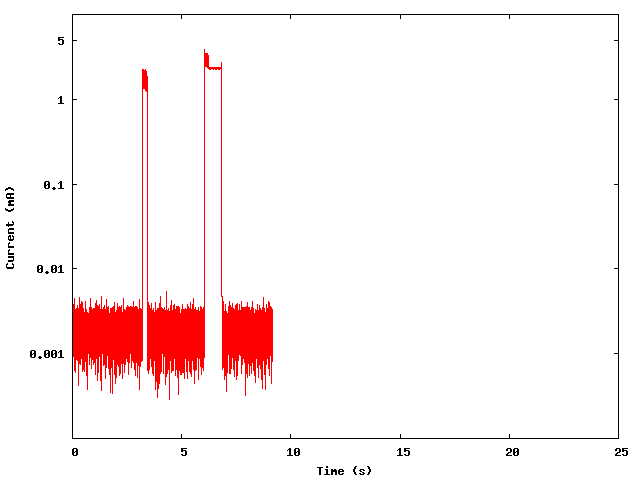
\includegraphics[width=0.75\textwidth]{data/play.png}
\caption{Playing power consumption}
\label{fig:playpower}
\end{figure}

\subsection{Holding}
When holding down a button, a peculiar pattern emerges (see figure \ref{fig:holdingpower}). 

There is a spike at first, then an intermediate energy level, before returning to EM2 energy consumption.

The intermediate energy level is explained by the fact that for an GPIO pin to receive power, this power has to come from somewhere. In fact, this power comes from the chip itself, as the pushing of the button closes a circuit, causing the system to draw power from itself.

While not a wanted feature, there's is nothing to do about this.

\begin{figure}[H]
\centering
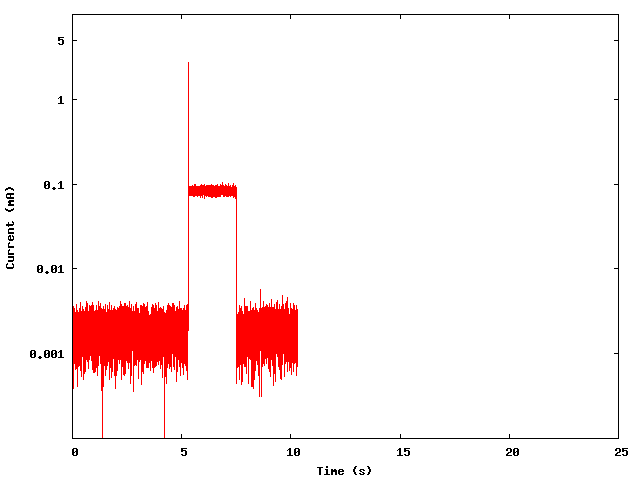
\includegraphics[width=0.75\textwidth]{data/hold.png}
\caption{Power consumption while holding button}
\label{fig:holdingpower}
\end{figure}
